% lista de exercícios 2 - teoria geral de sistemas

\documentclass[article,a4paper]{abntex2}
% \usepackage[a4paper,
%             includeheadfoot,
%             top=2cm,
%             right=2cm,
%             bottom=3cm,
%             left=3cm]{geometry}
\usepackage[OT1]{fontenc}
\usepackage{parskip}
\usepackage{graphicx}
\usepackage{enumitem}
\usepackage{pifont}
\usepackage{tikz}
\usetikzlibrary{calc, shapes}
\usepackage{amssymb}
\usepackage{amsmath}
\usepackage{hyperref} % cria os links de referencia das equacoes
% \usepackage[alf]{abntex2cite}
% \addbibresource{referencias.bib}

\begin{document}

\underline{\textbf{Resolução da Lista de Exercícios 2 - Ontologia de Sistemas}}\par
\textbf{Sistemas de Informação}\par
\textbf{Instituto Federal do Espírito Santo}\par
Campus Serra\par
\textbf{Teoria Geral de Sistemas}\par
Prof. Dr. Rodrigo Fernandes Calhau\par
Anderson A. Fraga (20222BSI0482)\par
\texttt{aafrg@tuta.io}\vspace{1cm}  %\texttt formats the text to a typewriter style font

Dada as referências \href{https://nemo.inf.ufes.br/wp-content/papercite-data/pdf/exploring_system_behavior_in_a_system_ontology_2023.pdf}{1} e \href{https://nemo.inf.ufes.br/wp-content/papercite-data/pdf/a_system_core_ontology_for_capability_emergence_modeling_2023.pdf#page=3.33}{2}, responda:
\begin{enumerate}
    \item \textbf{Defina "emergência" no contexto de sistemas.} \textit{Explique o que significa uma propriedade emergente e como ela se diferencia de uma propriedade resultante em um sistema, usando exemplos práticos.}
    \item \textbf{Explique o conceito de propriedade emergente no contexto de sistemas.} \textit{Use o exemplo do baú para descrever como as propriedades emergentes de "abertura" e "trancamento" do baú são geradas a partir de suas partes e disposições.}
    \item \textbf{Descreva como ocorre a emergência de novas propriedades em sistemas complexos.} \textit{Dê exemplos de sistemas físicos e sociais e explique como suas propriedades emergem das interações entre os componentes.}
    \item \textbf{Analise a relação entre a estrutura de um sistema e suas propriedades emergentes.} \textit{Use o exemplo de um sistema organizacional para discutir como a maneira pela qual os componentes estão conectados afeta o comportamento emergente.}
    \item \textbf{Descreva a diferença entre propriedades emergentes e propriedades resultantes.} \textit{Compare esses dois tipos de propriedades com exemplos do baú (como a "capacidade de abrir" do baú vs. a soma das massas das partes).}
    \item \textbf{Analise as relações entre propriedades (disposições) no exemplo do baú.}\textit{Discuta como as disposições do sistema (como a "capacidade de suporte" da base e a "revolubilidade" da tampa) são mutuamente ativadas e resultam na emergência de novas propriedades do baú. Explique como a "capacidade de trancar" da fechadura impede a "capacidade de abrir" do baú, discutindo o papel das disposições de "susceptibilidade ao trancamento" e "capacidade de trancar" no sistema.}
    \item \textbf{Elabore um Mapa Conceitual com base nos artigos definindo sistema e propriedades emergentes.}
    \item \textbf{Descreva como padrões de emergência podem ser identificados e replicados em sistemas sócio-técnicos.} \textit{Dê um exemplo de um sistema empresarial, como o caso do Spotify mencionado no documento, e explique como a identificação de padrões de emergência pode melhorar a adaptabilidade e a evolução da organização.}
\end{enumerate}\vspace{0.5cm}

Respostas:
\begin{enumerate}
    \item A emergência é definida como a propriedade que está relacionada as partes de um sistema e que, entretanto, não está presente separadamente e isoladamente em cada uma dessas partes. Um exmeplo de emergência é a propriedade de "flexibilidade" que uma cadeira carrega, porém, nem todas as partes dessa mesma cadeira podem conter a mesma flexibilidade quando analisadas separadamente.
    \item Assim, o conceito de propriedade de emergência se aplica quando há uma consequência direta da relação entre as partes de um sistema. As restrições que este mesmo sistema impõe formam situações onde as propriedades emergentes afloram. Como exemplo sugerido, um baú composto por uma estrutura em (1) madeira, com (2) molduras, (3) dobradiças, (4) os elementos fixadores como parafusos, e (5) tranca metálica, por meio da interação dessas mesmas partes, gera propriedades emergentes como a "abertura" e o "trancamento" do baú, com a interação entre todas as partes.
    \item A emergência de novas propriedades em sistemas complexos ocorre através de interações dinâmicas entre os componentes do sistema. As interações locais, auto-organização, diversidade e variedade de sistemas dão uma ideia sobre como essas propriedades surgem, como, por exemplo, em um sistema físico e social como em uma comunidade online onde as interações entre os usuários, como comentários, compartilhamentos e reações, criam um ambiente onde ideias e comportamentos podem se espalhar rapidamente. Essas interações levam à formação de normas sociais, modas e movimentos que emergem da colaboração e competição entre os indivíduos na plataforma.
    \item - 
    \item A principal diferença entre propriedades emergentes e resultantes é definida pelo imediatismo e nível de complexidade em que essas propriedades surgem. A propriedade emergente é marcada pelo surgimento quando não podem ser previstas ou deduzidas a partir das propriedades de suas partes individuais em um sistema, resultante de interações complexas entre os componentes do sistema; enquanto propriedades resultantes são previsíveis ou derivadas diretamente a partir das propriedades das partes do sistema, sendo o resultado da soma ou combinação das propriedades dos componentes. No exemplo sugerido, a capacidade de abrir o baú surge de interações simples de mais de um sistema - ser vivo que a abre e o sistema do próprio baú que possibilita essa propriedade; ao contrário da relação complexa entre as partes para que este movimento seja possível.
    \item -
    \item - 
    \item Os padrões de emergência são reproduzidos em sistemas socio-técnicos na medida em que as demandas exigem maior observação sobre detalhes que possam estar dificultando o desenvolvimento de atividades e produção dentro de uma organização. Identificar e reproduzir padrões exige o acompanhamento das interações presentes na empresa, entre os componentes sociotécnicos, de modo que seja possível a intervenção e modificação de componentes "destrutivos" em detrimento àqueles "construtivos" ao ambiente organizacional. Como exemplo, em uma pequena empresa de panificação, onde foi identificado que a produção diária de pães estava sendo afetada consistentemente por componentes responsáveis pela produção, o acompanhamento desses componentes e as interações entre eles e o ambiente são de grande importância para a alteração positiva da resolução do problema.
\end{enumerate}
    % \begin{figure}[!ht]
    %     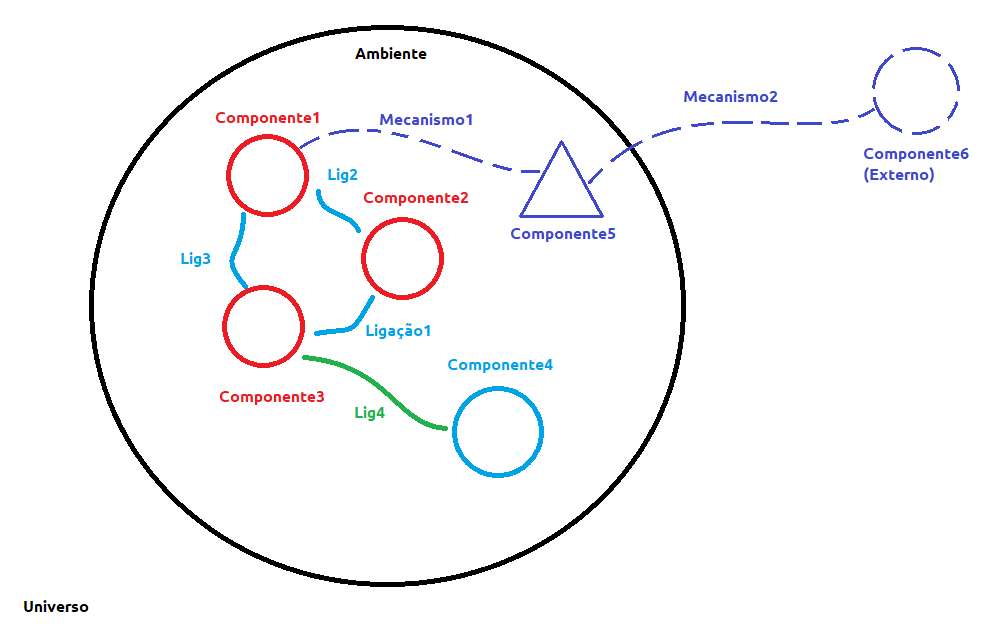
\includegraphics[width=16cm]{modeloConceitualCESM.png}
    % \end{figure}

\bibliography{referencias}

\end{document}